\section{Base\-Manager Class Reference}
\label{classBaseManager}\index{BaseManager@{BaseManager}}
Inheritance diagram for Base\-Manager:\begin{figure}[H]
\begin{center}
\leavevmode
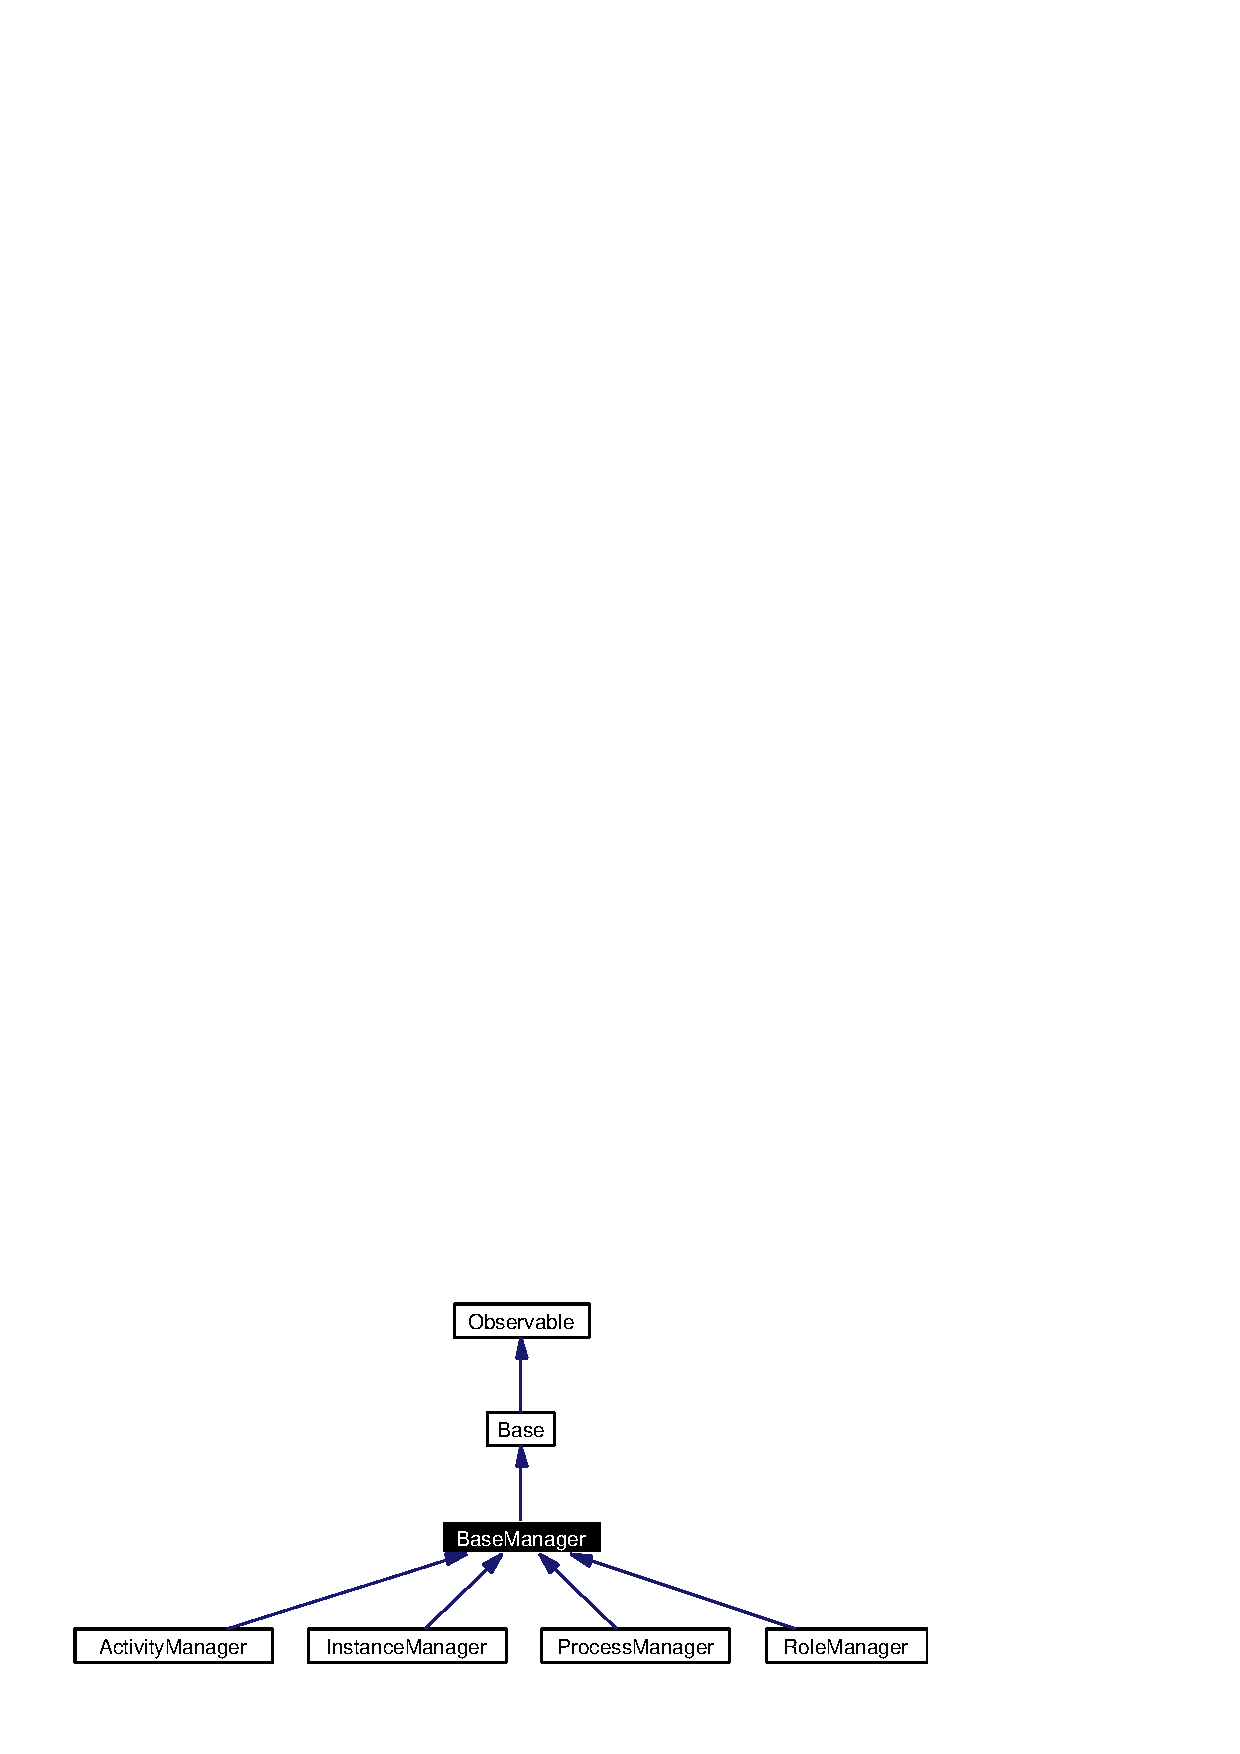
\includegraphics[width=222pt]{classBaseManager__inherit__graph}
\end{center}
\end{figure}
Collaboration diagram for Base\-Manager:\begin{figure}[H]
\begin{center}
\leavevmode
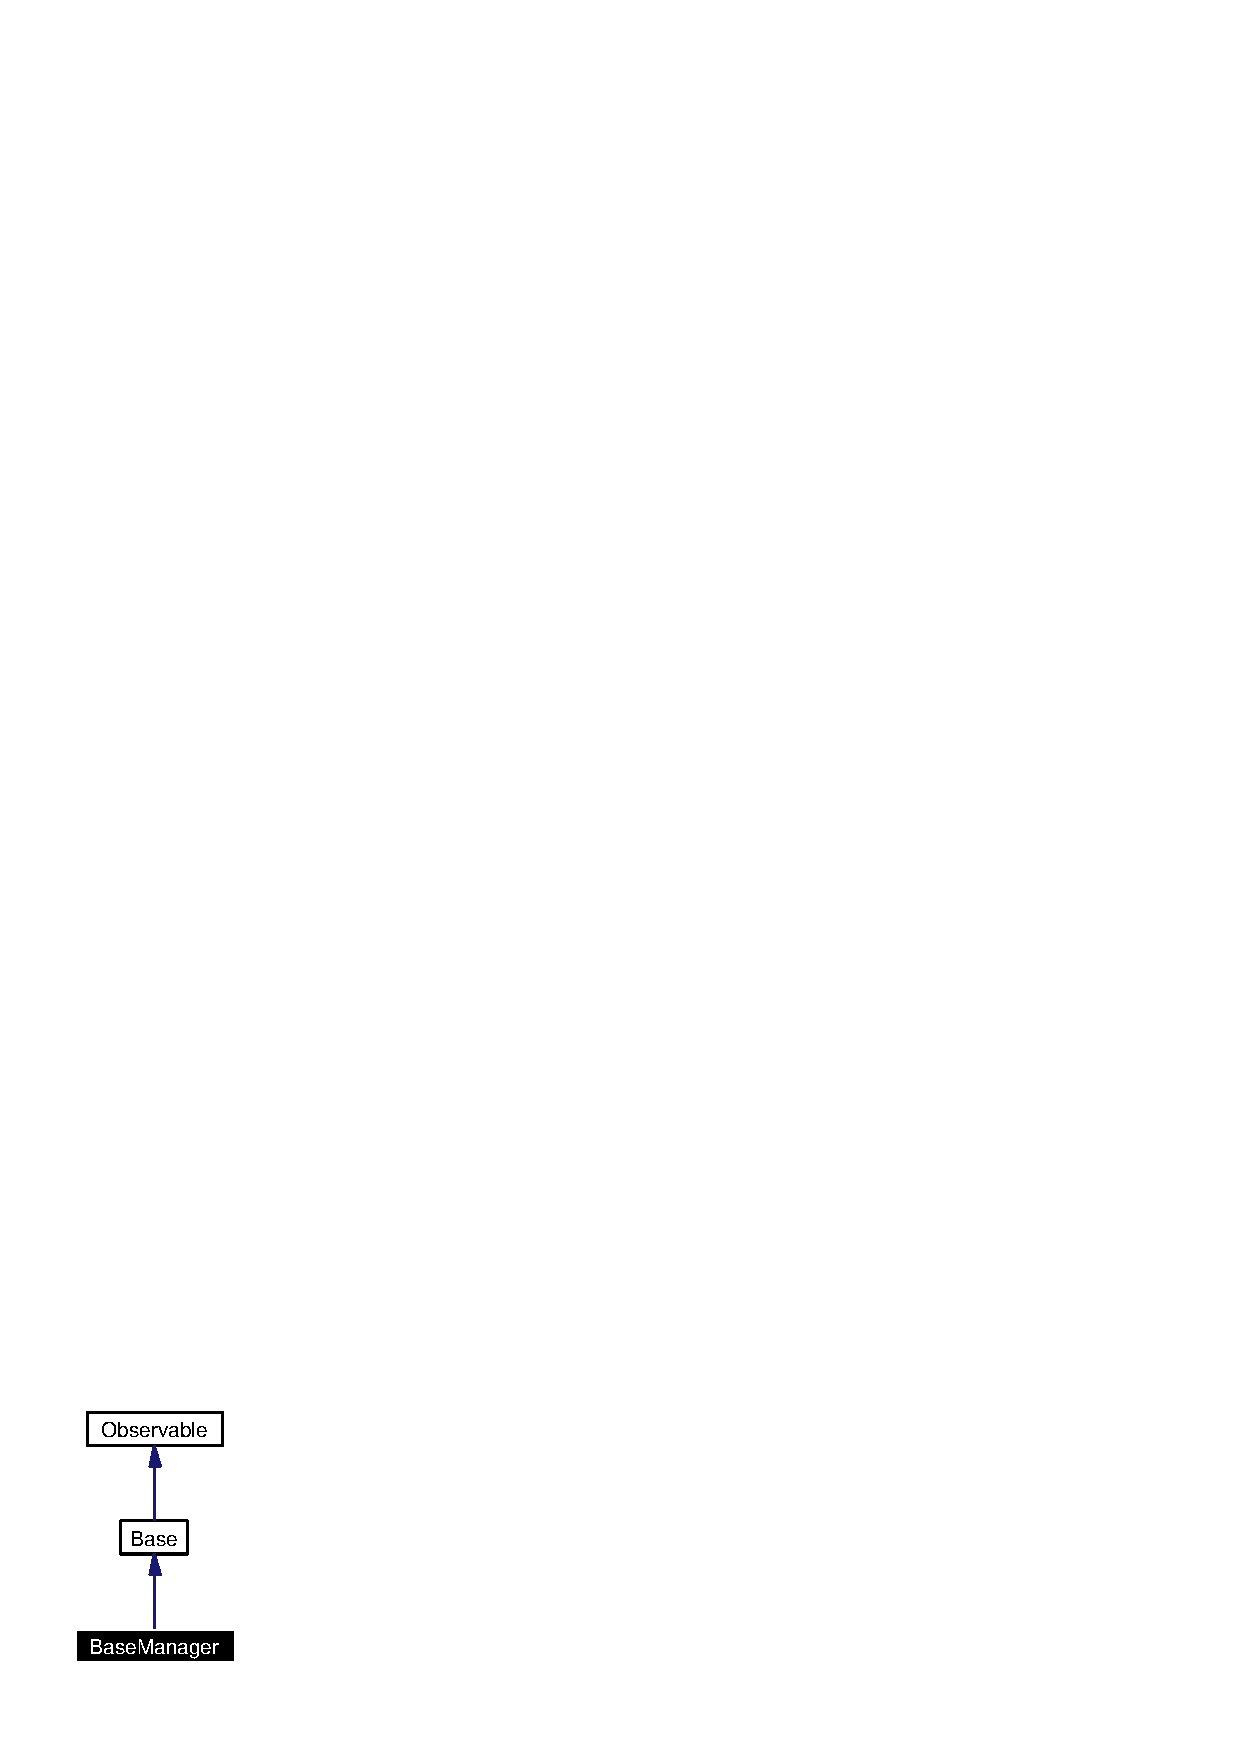
\includegraphics[width=56pt]{classBaseManager__coll__graph}
\end{center}
\end{figure}
\subsection*{Public Member Functions}
\begin{CompactItemize}
\item 
{\bf Base\-Manager} (\$db)\label{classBaseManager_a0}

\end{CompactItemize}


\subsection{Detailed Description}
This class is derived by all the API classes so they get the database connection, database methods and the {\bf Observable}{\rm (p.\,\pageref{classObservable})} interface. 



Definition at line 9 of file Base\-Manager.php.

The documentation for this class was generated from the following file:\begin{CompactItemize}
\item 
Base\-Manager.php\end{CompactItemize}
